\documentclass{article}
\usepackage[T1]{fontenc}
\usepackage{lmodern}
\usepackage{graphicx}
\usepackage{amsmath,amssymb}
\usepackage[a4paper,margin=2cm]{geometry}
\usepackage[absolute,overlay]{textpos}
\setlength{\TPHorizModule}{1mm}
\setlength{\TPVertModule}{1mm}
\usepackage[indonesian]{babel}
\usepackage{hyperref}
\setlength{\emergencystretch}{2em}
% unit: Halaman 48

\begin{document}

% === Halaman 48 (llm) ===

\vspace{172.26mm}

Sumber: William Stalling, Cryptography and Network Security\nOverview & Chapter 1

\vspace{60mm}

\begin{center}
\textbf{Active Attack: Modification}
\end{center}

% deskripsi: Diagram yang mengilustrasikan serangan aktif berupa modifikasi pesan, di mana penyerang bernama Darth mencegat dan mengubah pesan yang dikirim oleh Bob kepada Alice melalui internet atau fasilitas komunikasi lainnya.
% bbox normalisasi: [0.1700, 0.1500, 0.8300, 0.7300]
\begin{textblock*}{138.60mm}(35.70mm,44.55mm)
\noindent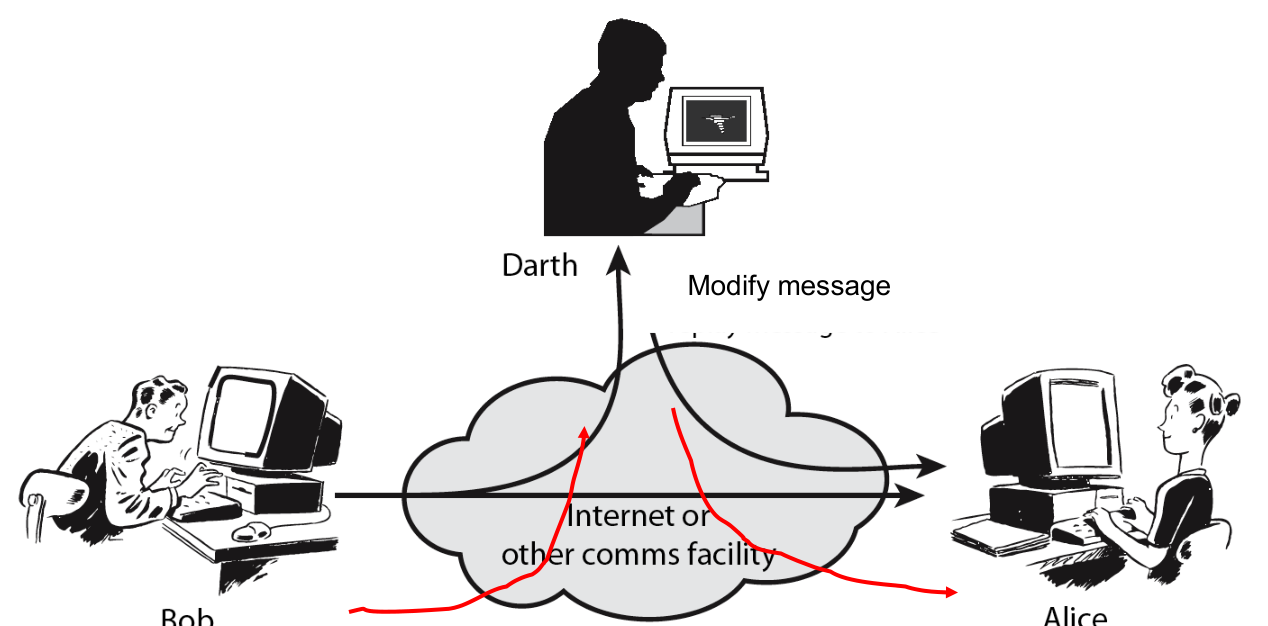
\includegraphics[width=138.60mm,height=172.26mm]{../../images/llm/page_048_img_01.png}%
\end{textblock*}

\end{document}
